%% For double-blind review submission, w/o CCS and ACM Reference (max submission space)
\documentclass[acmsmall,screen,anonymous,nonacm]{acmart}\settopmatter{printfolios=true,printccs=true,printacmref=true}
%% For double-blind review submission, w/ CCS and ACM Reference
%%\documentclass[acmsmall,review,anonymous]{acmart}\settopmatter{printfolios=true}
%% For single-blind review submission, w/o CCS and ACM Reference (max submission space)
%\documentclass[acmsmall,review]{acmart}\settopmatter{printfolios=true,printccs=false,printacmref=false}
%% For single-blind review submission, w/ CCS and ACM Reference
%\documentclass[acmsmall,review]{acmart}\settopmatter{printfolios=true}
%% For final camera-ready submission, w/ required CCS and ACM Reference
%\documentclass[acmsmall]{acmart}\settopmatter{}

%%%%%%%%%%%%%%%%%%%%%%%%%%%%%%%%%%%%%%%%%%%%%%%%%%%%%%%%%%%%%%%%%%%%%%
%% Note: Authors migrating a paper from PACMPL format to traditional
%% SIGPLAN proceedings format must update the '\documentclass' and
%% topmatter commands above; see 'acmart-sigplanproc-template.tex'.
%%%%%%%%%%%%%%%%%%%%%%%%%%%%%%%%%%%%%%%%%%%%%%%%%%%%%%%%%%%%%%%%%%%%%%

%% Title information
\newcommand{\thetitle}{How to Evaluate Blame for Gradual Types}
\title{\thetitle}

%% Author information
%% Contents and number of authors suppressed with 'anonymous'.
%% Each author should be introduced by \author, followed by
%% \authornote (optional), \orcid (optional), \affiliation, and
%% \email.
%% An author may have multiple affiliations and/or emails; repeat the
%% appropriate command.
%% Many elements are not rendered, but should be provided for metadata
%% extraction tools.

\author{Nobody In Particular}
% \affiliation{\institution{PLT} \city{Evanston} \country{Illinois} }
\affiliation{\relax} % \institution{PLT} \city{Evanston} \country{Illinois} }
% \email{chrdim@northwestern.edu}          %% \email is recommended



\usepackage{alltt}
\usepackage{wrapfig}

%% Some recommended packages.
\usepackage{booktabs}   %% For formal tables:
                        %% http://ctan.org/pkg/booktabs
\usepackage{subcaption} %% For complex figures with subfigures/subcaptions
                        %% http://ctan.org/pkg/subcaption

\usepackage{listings}
\usepackage[shortcuts]{extdash}
\usepackage{xcolor}

\usepackage{upgreek}

%\usepackage{draftwatermark}
%\SetWatermarkText{DRAFT}
%\SetWatermarkScale{1}


%%%%%%%%%%%%%%%%%%%%%%%%%%%%%%%%%%%%%%%%%%%%%%%%%%%%%%%%%%%%%%%%%%%%%%%%%%%%%%%%%%%%%%%%%%%%
%%%%%%%%%%%%%%%%%%%%%%%%%%%%%%%%%%%%%%%%%%%%%%%%%%%%%%%%%%%%%%%%%%%%%%%%%%%%%%%%%%%%%%%%%%%%
%%%%%%%%%%%%%%%%%%%%%%%%%%%%%%           PREAMBLE       %%%%%%%%%%%%%%%%%%%%%%%%%%%%%%%%%%%% 
%%%%%%%%%%%%%%%%%%%%%%%%%%%%%%%%%%%%%%%%%%%%%%%%%%%%%%%%%%%%%%%%%%%%%%%%%%%%%%%%%%%%%%%%%%%%
%%%%%%%%%%%%%%%%%%%%%%%%%%%%%%%%%%%%%%%%%%%%%%%%%%%%%%%%%%%%%%%%%%%%%%%%%%%%%%%%%%%%%%%%%%%%

% acmart formatting
\settopmatter{printfolios=true}
\overfullrule=1mm

% techreport title
\newcommand{\techreport}{supplementary material}

% short url formatting
\newcommand{\shorturl}[2]{\href{#1#2}{\texttt{#2}}}

%%%%%%%%%%%%%%%%%%%%%%%%%%%%%%%%%%%%%%%%%%%%%%%%%%%%%%%%%%%%%%%%%%%%%%%%%%%%%%%%%%%%%%%%%%%%
%%%%%%%%%%%%%%%%%%%%%%%%%%%%%%%%%%%%%%%%%%%%%%%%%%%%%%%%%%%%%%%%%%%%%%%%%%%%%%%%%%%%%%%%%%%%
%%%%%%%%%%%%%%%%%%%%%%%%%%%%%%%%%%%%%%%%%%%%%%%%%%%%%%%%%%%%%%%%%%%%%%%%%%%%%%%%%%%%%%%%%%%%


%% lattice

\newcommand{\system}{\ensuremath{P}}



\newcommand{\component}{\ensuremath{c}}

\newcommand{\latticeL}{\mathcal{L}}

\newcommand{\lattice}[1]{\ensuremath{\latticeL\llbracket#1\rrbracket}}

\newcommand{\standardlattice}{\lattice{\system}{\kmap}}

\newcommand{\conf}{\ensuremath{s}}

\newcommand{\metric}{\ensuremath{\leq_{\latticeL}^{X}}}

\newcommand{\set}[1]{\ensuremath{\bar{#1}}}

\newcommand{\size}[1]{\ensuremath{\mid #1 \mid}}

\newcommand{\blame}[1]{\ensuremath{blame\llbracket#1\rrbracket}}

\newcommand{\mblame}[1]{\ensuremath{multiblame\llbracket#1\rrbracket}}



\newcommand{\faulty}[1]{\ensuremath{FAULTY\llbracket#1\rrbracket}}

\newcommand{\random}[1]{\ensuremath{random\llbracket#1\rrbracket}}

\newcommand{\error}[1]{\ensuremath{error\llbracket#1\rrbracket}}

\newcommand{\effort}[1]{\ensuremath{EFFORT\llbracket#1\rrbracket}}

\newcommand{\first}[1]{\ensuremath{first\llbracket#1\rrbracket}}

\newcommand{\last}[1]{\ensuremath{last\llbracket#1\rrbracket}}


\newcommand{\modem}{\ensuremath{S}}
\newcommand{\mode}[1]{\ensuremath{\modem\llbracket#1\rrbracket}}





%% misc

\newcommand{\setsize}[1]{\left|#1\right|}

\newcommand{\codesize}{\small}

\newcommand{\codecolor}{black}

\let\OldTexttt\texttt
\renewcommand{\texttt}[1]{\OldTexttt{\color{\codecolor}{#1}}}

\let\Oldtt\tt
\renewcommand{\tt}{\Oldtt \color{\codecolor} }

\newcommand{\todo}[1]{{\textcolor{red}{TODO}\{\textcolor{gray}{#1}\}}}

\newenvironment{code}{\codesize \color{\codecolor} \begin{alltt}}{\end{alltt}}


%% %%%%%%%%%%%%%%%%%%%%%%%%%%%%%%%%%%%%%%%%%%%%%%%%%%%%%%%%%%%%%%%%%%%%%%%%%%%%%
%% for leaving margin notes in the paper write
%% \yourinitials{...} 

\def\notes#1{\expandafter\def\csname#1\endcsname##1{\marginpar{\raggedright\tiny $\bullet$ #1 says: ##1}}}
\notes{mf}
\notes{cd}
\notes{ll}
\notes{bg}


%% Journal information
%% Supplied to authors by publisher for camera-ready submission;
%% use defaults for review submission.
\startPage{1}

%% Copyright information
%% Supplied to authors (based on authors' rights management selection;
%% see authors.acm.org) by publisher for camera-ready submission;
%% use 'none' for review submission.
%% \setcopyright{none}
%\setcopyright{acmcopyright}
%\setcopyright{acmlicensed}
%\setcopyright{rightsretained}
%\copyrightyear{2018}           %% If different from \acmYear

%% Bibliography style
\bibliographystyle{ACM-Reference-Format}
%% Citation style
%% Note: author/year citations are required for papers published as an
%% issue of PACMPL.
\citestyle{acmauthoryear}   %% For author/year citations

%%%
\setcopyright{none}
\acmPrice{1}
\acmDOI{}
\acmYear{}
\copyrightyear{}
\acmJournal{pacmpl}
\acmVolume{1}
\acmNumber{1}
\acmArticle{1}
\acmMonth{1}


\begin{document}

%% Abstract
%% Note: \begin{abstract}...\end{abstract} environment must come
%% before \maketitle command
\begin{abstract}
Gradual types and blame go hand in hand. But what is the value of blame?
\end{abstract}



% CCS concepts: Program specifications < Program reasoning < Semantics and Reasoning < Theory of Computation
% CCS concepts: Empirical software validation < Software verification and validation < Software creation and management < Software and its engineering

% potential choices decided against: pre- and post-conditions, assertions, software testing and debugging

%\begin{CCSXML}
%<ccs2012>
%<concept>
%<concept_id></concept_id>
%<concept_desc></concept_desc>
%<concept_significance></concept_significance>
%</concept>
%<concept>
%<concept_id></concept_id>
%<concept_desc></concept_desc>
%<concept_significance></concept_significance>
%</concept>
%</ccs2012>
%\end{CCSXML}

%\ccsdesc[]{}
%\ccsdesc[]{}


%% Keywords
%% comma separated list
%\keywords{}  %% \keywords are mandatory in final camera-ready submission


%% \maketitle
%% Note: \maketitle command must come after title commands, author
%% commands, abstract environment, Computing Classification System
%% environment and commands, and keywords command.
\maketitle

\section{Does Blame Matter?} \label{sec:introduction}

Theoreticians of gradual typing have focused on
blame theorems from the very beginning~\cite{mf-toplas-2009, tf-dls-2006}. ``Well-typed
[components]\footnote{The original authors got this word wrong.} can't be
blamed'' turned the theorem into a slogan~\cite{wf-esop-2009}. Indeed,
academic implementations---for example, Reticulated
Python~\cite{vsc-dls-2019, vss-popl-2017, vksb-dls-2014} and Typed
Racket~\cite{tf-dls-2006,tf-popl-2008,tfffgksst-snapl-2017,tf-icfp-2010}---come
with sophisticated blame assignment strategies. The academics that
created them firmly embrace the idea that blame can help practicing
programmers find impedance mismatches between the types they added to a
software system and the behavior of the remaining untyped components. 

Industrial implementors of  gradual typing systems have almost completely ignored blame assignment.
Systems such as Flow,\footnote{\url{https://flow.org}}
Hack,\footnote{\url{https://hacklang.org}} or
TypeScript\footnote{\url{https://www.typescriptlang.org}} exploit types for IDE actions and for finding typos in
code. Then their compilers remove types and rely on the built-in safety checks of
the underlying programming language to catch any problems. 
Recently, \citet{cc-snapl-19} have turned this implicitly expressed
skepticism into an explicit statement and challenge.

This contrast between theoretical research and industrial applications of gradual typing raises the question 
\begin{quote}
 \it
 whether blame assignment adds any value to a gradually typed language, \\
 especially for the benefit of the working programmer.
\end{quote}
Given the long standing academic interest in blame  and its complete absence in
industrial systems, it comes as an even bigger surprise that the research
literature and the industrial blog world do not present or discuss any
possible answers.  Instead, when language designers decide to look into the
question, they seem to answer it one way or another without any scientific
justification. As a matter of fact, the research community simply does not have a
method for evaluating blame, and given the question's practical
relevance, this a significant problem.

This paper's first contribution is an automated method for evaluating the
effectiveness of blame assignment strategies in the gradual typing world.
%% (sections ~\ref{sec:landscape},~\ref{sec:mutate},~\ref{sec:rational} and \ref{sec:sample}). 
%% MF: says you can't simulate a roadmap by listing all sections.
%% MF: and for heaven's sake lookup the use of ~ in TeX
Roughly speaking, the method, which is
loosely based on the work of Lazarek et al.~\cite{lksfd-popl-2020},
simulates a programmer who follows the Wadler-Findler slogan quoted above.
Such a \emph{rational programmer} can find impedance-mismatch
bugs by adding types to a partially typed program (section~\ref{sec:landscape}). That is, when the
run-time system signals an impedance mismatch, a good blame message helps
the programmer infer where to add an additional type specification. Since
components that pass the type checker cannot cause impedance mismatches;
the type checker discovers these mismatches at compile time and points
directly to the faulty component. Otherwise, if the
additional type does {\em not\/} cause a static type error, the program
 is run again to signal another violation. Then the programmer can heed
blame one more time to add yet another type specification. Weighing the number of
steps it takes to discover the mistake in this manner is a measure of the effectiveness
of the blame assignment strategy of the language.

The paper's second contribution is a set of results from applying the evaluation
method to three distinct blame assignment strategies and approximately 20,000
cases\mf{Replace with real number} (section~\ref{sec:results}): Vitousek et
al.'s strategy of tracking typed/untyped boundaries in Reticulated;
Tobin-Hochstadt et al.'s use of higher-order contract system~\cite{ff-icfp-2002,
mf-toplas-2009}; and the approach of industrial systems that forego blame
and instead rely on error messages from the
underlying programming language.

\mf{This is made up and must be fixed for the submission.}

A direct interpretation of the results (section~\ref{sec:discussion}) is that
they validate the conjecture behind the work of theoreticians. A good blame assignment
strategy
greatly shortens the search for impedance mismatches between the specified types
and the behavior of untyped components. Even better, the evaluation method clearly
identifies the wrapper-based blame tracking of Typed Racket as the vastly superior
academic system. Vitousek et al. lose one more time. Of course, a detailed
discussion must acknowledge the threats to validity of these results.

Next, the paper describes the challenges of developing an evaluation
method, which may explain why the question has been neglected for such
a long time.


 \label{sec:introduction}
%% -----------------------------------------------------------------------------
\def\fname#1#2{$\underline{\hbox to #2in{#1}}$\\[-2ex]}

\begin{figure*}[hbt]\footnotesize
  \vspace{-1mm}

\begin{minipage}[t]{2.2in}
\begin{alltt}\fname{untyped/pack-lib}{1.8}
(provide pack _ _ _)

_ _ _  dependencies     _ _ _
_ _ _  and definitions  _ _ _

(define (pack d)
  ;; process JSON data and 
  ;; package it in a dictionary
  ;; (association list)
  (make-hash _ _ _) ;; BUG!)


\end{alltt}
\end{minipage}\begin{minipage}[t]{2.2in}
\begin{alltt}\fname{typed/pack-lib}{1.7}
(provide typed-pack)

(require/typed pack-lib
  [pack 
  (-> JSON 
      (Listof 
       (Pairof Symbol String)))])

(define typed-pack pack) 
\end{alltt}
\smallskip
\begin{alltt}\fname{typed/crypto-pack-lib}{1.7}
(provide crypto-pack) 

(require/typed pack-lib
 [pack 
  (-> JSON 
      (Listof 
       (Pairof Symbol String)))])

(define (crypto-pack [d : JSON])
  (pack (encrypt d _ _ _)))

 \end{alltt}
\end{minipage}\begin{minipage}[t]{2.2in}
\begin{alltt}\fname{untyped/client}{1.65}
(require json 
         typed/pack-lib
           typed/crypto-pack-lib)

_ _ _  other dependencies  _ _ _
_ _ _  and definitions     _ _ _
          
;; read data from files, pack 
;; and share securely 

(define public-data 
  (typed-pack 
   (read-json 
    "public-records")))

(define secret-data 
  (crypto-pack 
   (read-json 
    "medical-records")))
 
 _ _ _ rest of client _ _ _
\end{alltt}\end{minipage}

   \caption{One mix-typed program, three interpretations} \label{fig:example}

  \vspace{-1mm}
\end{figure*}
%% -----------------------------------------------------------------------------

The program sketch in figure~\ref{fig:example} demonstrates the
differences between Natural, Transient and Erasure using Typed Racket
syntax.  The modules on the left and right are untyped while the two
in the middle are typed.

The \texttt{untyped/pack-lib} module (left) provides, among others, a function
\texttt{pack} that consumes JSON data and packages it in a dictionary. However,
by mistake \texttt{pack} returns a hash table instead of the association list
its documentation promises.  The \texttt{client} module (right) uses
\texttt{pack} indirectly to package public and sensitive data it reads from the
filesystem. It does so through two different intermediary typed modules
(center). The first, {\tt typed/pack-lib}, imports \texttt{pack} and re-exports
it as \texttt{typed-pack} asserting that it is a function that consumes {\tt
JSON} and returns a list associating {\tt Symbol}s with {\tt String}s. The
second typed module, {\tt typed/crypto-pack-lib}, also imports \texttt{pack} and
assumes for it the same type as {\tt typed/pack-lib}. Instead of exporting it,
it uses the function in the exported {\tt crypto-pack} function, which encrypts
its input before passing it to \texttt{pack}.

Under the {\it Natural\/} semantics~\cite{tf-popl-2008,tfffgksst-snapl-2017},
functions imported into and exported from typed modules are wrapped in proxies
that enforce the static type discipline with run-time checks and track
responsibilities. Thus, when \texttt{pack} is imported into a typed module, the
run-time system checks that it is a function and wraps it in a protective proxy,
which in turn, enforces the type of the function with run-time checks.  In
essence, this check protects typed modules when they call an untyped function
because it may not produce the promised kind of value, as is the case here with
{\tt pack} from {\tt untyped/pack-lib}. Analogously the run-time system wraps
exported functions such as {\tt crypto-pack} of a typed modules in a proxy that
checks its arguments.  This check protects functions exported from type modules
against applications in untyped code that supply the wrong kind of argument
value.

As this analysis implies, if the return-type check fails, the problem is with
the untyped module that supplied an incorrect function, here {\tt
untyped/pack-lib}. If the argument-type check fails, responsibility lies with
{\tt client}. Due to the proxies wrapped around functions, Natural can easily
track the responsible party for each check. Thus, in the example of
figure~\ref{fig:example}, as \texttt{typed-pack} returns, the return-type check
fails, and Natural blames \texttt{pack-lib}.

Under the Transient semantics~\cite{vss-popl-2017}, typed code is compiled so
that all entry points to functions check their arguments at run time and all
function calls check their return values against the expected type.
Furthermore, Transient uses \emph{shallow} checks, meaning they check only the
top constructor of a value. Since retrieving a value from within a structure (or
list, array, hash table etc.) is performed via a function call, the innards of a
complex value are checked on a piecemeal basis.

As a result, the call to \texttt{typed-pack} does not signal an error because
the call takes place in the untyped {\tt client} module, which is compiled in
the usual manner. Because {\tt pack} is called in the {\tt
typed/crypto-pack-lib} module, Transient's inlined checks make sure that the
imported \texttt{pack} is a function and that the result of its call in is a
list. This last check fails when \texttt{client} calls to {\tt crypto-pack}.

In order to pinpoint the responsible party for failed checks, Transient
maintains a map from values to the boundaries between typed/untyped modules that
they cross, plus the corresponding types. In the example, the map records that
\texttt{pack} crosses from \texttt{untyped/pack-lib} to {\tt typed/pack-lib} and
from {\tt typed/pack-lib} to {\tt client} with the type that appears in the {\tt
required/typed} forms in the example. Since the failed check corresponds to the
return type of \texttt{pack}, Transient blames the sources of the two boundary
crosses, which in this particular case is \texttt{untyped/pack-lib} for both. In
general though, Transient blames more than one party. In fact, the theoretical
work of~\citet{gfd-oopsla-2019} shows that for some programs Transient
constructs a blame set that excludes responsible parties and includes modules
irrelevant to the failing check.

Under the Erasure semantics, the compiler checks the specified types and then
discards them when it generates code. The generated code includes run-time
checks that ensure the dynamic safety of all operations as specified in the
underlying untyped language. Hence, neither the call to {\tt typed-pack} nor the
call to {\tt crypto-pack} signals an error due to the gradual type system.

When run, the program may raise an exception if \texttt{client} tries to
inspect the elements of the list that \texttt{typed-pack} and
\texttt{crypto-pack} are supposed to produce. The information in this exception,
plus its stack trace, or may not help the programmer find the source of the
impedance mismatch between the specified return types of {\tt pack} in the two
typed modules and the actual return value of {\tt pack}.

All three systems used here are implemented on top of the common basis of
Racket. The use the Typed Racket syntax and type checker for all three
semantics. The Natural semantics is inherited as is, while the Erasure semantics
is the one of plain Racket.  The Transient system implements the design
of~\citet{vss-popl-2017}, though constructing it demands two design decisions:
which shallow checks to use and where, plus how to maintain a blame map in a
full-fledged run-time system. 

For certain types, such as {\tt String} or {\tt (Vectorof Byte)}, Transient can
realize shallow checks with the predicate from Racket.  Other types require
custom predicates; for example the type {\tt Index} of valid array indices
allows a range of positive exact integers.  Many custom predicates run in
constant time, but some, such as the one for {\tt (Union T1 ... Tn)}, run in
linear time. The key point is that no shallow check inspects beyond the top
constructor of each type.

Once the type checker has completed its work, Transient translates the source
into an alternative form and in the process inserts run-time checks. Technically
speaking, the rewriting pass wraps all elimination in applications of shallow
checks.  For example, if the variable {\tt f} has the static type {\tt (->
String String)}, the application {\tt (f x)} must be rewritten to check for a
string result because {\tt f} could be an untyped function.

The rewriting pass also inserts hooks for updating the blame map.  When a value
crosses a module boundary, such a hook records a type assumption in the blame
map.  The in-lined checks for elimination forms extend the blame map with
further information. For instance, the check of the result of {\tt (f x)} adds
an entry to the blame map that records the expected type of the result as the
return type of the type of {\tt f}.  If a Transient check ever fails, the
run-time checking system of Transient Racket walks over the information in the
blame map and reports a sequence of blamed components.

%% MF: I have no clue what the following contributes: 

% \smallskip
% \noindent
% {\bf Note.} As the common basis for the three semantics, we choose Typed
% Racket's migratory typing. In contrast to the initial formulation of gradual
% typing~\cite{st-sfp-2006}, migratory typing does not provide support for type
% \texttt{Dyn}, components are either untyped or fully typed.
% %% MF: does it ever:
% %% and the gradual type system does not affect the compilation of untyped components. 
% Despite, these differences, Typed Racket is the most
% mature system for sound mix-typed code
% and recent theoretical work has established that
% its migratory typing offers a setting for comparing different approaches to gradual
% typing~\cite{gf-icfp-2018,gfd-oopsla-2019}.
    \label{sec:landscape}
\section{Why Is It Hard to Evaluate Blame?}
\label{sec:challenges}

%% -----------------------------------------------------------------------------

The general challenge of evaluating blame is a methodological one. Unlike most
current research on programming languages, the question seems to call for
empirical research similar to that of human-computer interaction. At the same
time, a significant evaluation result demands a large number of cases yielding a
serious amount of data. As~\citet{lksfd-popl-2020} recently demonstrated, the
way around this dilemma is to postulate the equivalent of a {\it homo
economicus\/} for programming languages---the {\em rational programmer\/}---and
to implement this rational programmer as an algorithm.

In the context of gradual typing, the rational programmer translates the
Wadler-Findler slogan into a debugging method, searching for the source of the
impedance mismatch in an incremental fashion. Measuring this simulated
programmer's behavior on a large number of debugging sessions yields data that
is similar to data collected in an empirical, human-facing manner.

The {\em first derivative challenge\/} is to find a representative collection of
impedance mismatches between typed and untyped pieces of code that programmers
may accidentally create and that the run-time checks of academic systems
catch. In other words, the experiment calls for a collection of type mistakes in
mix-typed programs that is representative of those ``in the wild.''
Unfortunately no such collection exists, and with good reason. The kind of
mistakes needed are typically detected by unit or integration tests; even if it
takes some time to find their sources, these mistakes do not make it into code
repositories with appropriate commit messages.

Following~\citet{lksfd-popl-2020} again, the alternative is to {\em generate a
sufficiently large and representative corpus of type mistakes \/} using mutation
analysis~\cite{lipton1971fault, demillo1978hints, jia2011analysis}.  The
mutation analysis of Lazarek et al, is, however, useless for creating impedance
mismatches.  While mutation analysis traditionally aims to inject bugs that
challenge test suites, it discards those that yield ill-typed mutants as
\emph{incompetent}.  Indeed, mutation analysis frameworks are fine-tuned to
avoid them---and yet it is precisely those that are needed for evaluating blame
assignment strategies.

Thus, an experimental analysis of blame needs a mostly new set of mutators.
Roughly speaking, the new mutators inject type errors into fully typed programs.
Applying such a mutator to any typed component produces a mutatnt component.  A
debugging scenario results from removing the types from the mutatnt. For the
design of such mutators, the authors relied on their own extensive programming
experience though not without discovering a major pitfall: some of their
original mutators systematically produced programs that immediately revealed the
source of the impedance mismatch. About two thirds of the original mutators
survived this first scrutiny testing. All of the remaining ones yield
interesting (see section~{sub:interesting}) debugging sessions.

The {\em second derivative challenge\/} concerns the differences among the blame
assignment of the three semantic variants.  While Natural assigns blame to {\em
one\/} component, Transient assigns blame to a sequence of components. The
Erasure semantics does not blame a component {\it per se\/}, but it comes with
an exception location and a stack trace, which implicitly suggests parties to
blame.  The different strategies greatly affect the behavior of the rational
programmer (and real programmers, too).

One way to overcome this challenge is to equip the rational programmer with
\emph{modes} that represent the alternative interpretations of blame.  For
instance, a mode of the rational programmer using Transient may pick the oldest
element of a blame set as the next component to add types because it corresponds
to the earliest point in the program's evaluation that can discover an impedance
mismatch.  Another mode may opt to treat the blame set as another form of a
stack trace and add types to its newest element.  When both modes are equally
successful in locating an impedance mismatch, the method can measure the
rational programmer's effort to answer which mode is the most effective.

Different blame information is also due to differences in the run-time checks
that the three gradual typing systems perform. This observation suggests another
mode for the rational programmer, namely, a mode that ignores the blame
information completely and instead inspects only the information in the
exceptions of the safety checks in the underlying languages.  This
\emph{exception} mode serves as the baseline for blame's value; if the
programmer in this mode ``beats'' the others, blame systems might be useless. 

The {\em third challenge\/} is the explosion of debugging scenarios that results
from the combination of mutation-based scenario generation and mode-based
analysis. All three factors---three different gradual typing systems, the large
number of mutants, and the number of debugging modes---contribute possibly
useful debugging data in multiplicative manner. Hence, carried out naively, the
experiment would demand an unacceptably large amount of computational resources.
A practical execution has no option but to sample the space of scenarios,
carefully ensuring that it still produces reproducible conclusions.

Overcoming these challenges needs a systematic approach: 
\begin{itemize}

\item a suitable set of mutators for the generation of interesting type-level
 errors (section~\ref{sec:mutate});
    
\item an algorithmic simulation of the many modes of the rational programmer on
 the corresponding debugging scenarios (section~\ref{sec:rational});

\item a careful sampling of the space (section~\ref{sec:sample}).
\end{itemize}
Getting all three aspects right is necessary to obtain a computationally
feasible and statistically sound experiment

{\bf Note} A somewhat coincidental challenge is the disparity of gradually typed
languages. While the three approaches to blame are well understood in theory,
they have been implemented for rather different untyped languages and with
vastly different type systems. To eliminate the effect of these differences, it
is necessary to implement all three approaches in a single language so that an
application of an evaluation method can use the same test programs, the same
type system, and hence the same debugging scenarios.

The results in this paper are for a system that builds on Greenman and
Felleisen's effort comparing the performance of Natural and Transient in
Racket~\cite{gf-icfp-2018}. The extended system uses the type system of Typed
Racket and comes with a Transient semantics that is comparable with the Natural
one. The Transient semantics of the system also realizes the design of the blame
assignment system proposed by~\cite{vss-popl-2017}. The Erasure semantics drops
the type information and runs the programs as if they were plain Racket
programs. The next section explains this system in detail.
   \label{sec:challengs}
\section{How to Simulate the Rational Programmer} \label{sec:ideas}

Given the comparable implementations of the three gradual typing systems,
the next step for applying our method is to obtain a set of fully
typed benchmarks that each comes with a single impedance mismatch between
its type specifications and its code. As we briefly discuss in
section~\ref{sec:challenges}, we derive such ill-typed benchmarks with
mutation analysis from well-typed programs.  We return to mutation
analysis and the benchmarks in section~\ref{sec:experiment}.  Herein,
we assume that we have them in hand and instead we focus on the
main element of our method, the rational programmer.  


The rational programmer exploits blame information to figure out wih. Therefore the way to understand its behavior 
is to analyze the migratory path it follows through the 
\emph{configuration space} of the program. The space
consists of variants of the program, dubbed \emph{configurations}, that 
differ in their type annotations. 
Herein we build on top of Typed Racket's migratory typing
approach,\footnote{The method can be adapted to so-called true gradual typing
systems~\cite{svcb-snapl-2015} in a straightforward manner.}, hence, each configuration differs from another
in which of its components are typed and which are not. Formally, we can
represent a program $\system$ as a set of of components
$\set{\component}$ and each configuration $\conf$ of $\system$ is a subset of 
$\set{\component}$
that contains exactly the components of  $\system$ that are typed in
$\conf$. Naturally the configurations of  $\system$ are ordered by the subset relation and
thus form a lattice $\lattice{\system}$ with size $2^{\size{\system}}$.
The bottom configuration of $\lattice{\system}$ is always $\emptyset$ and
the top element is $\system$ itself. In between there are all the
mixed-type configurations. If we assume that  component $\component$ of $\system$
contains the type error, any configuration $\conf$ that
includes $\component$ is ill-typed. Any other configuration $\conf$ may blame 
a $\component_b$, which we denote with $\blame{\conf}$. Let a blametrail
be a sequence of configurations $\conf_0,...\conf_n$ where 
for all $0 \leq i \leq n - 1$, $\conf_i \subset \conf_{i+1}$ and
$\conf_{i+1} \setminus \conf_i = \blame{\conf_i}$. That is a blametrail
corresponds to a succession of a configurations that start with a
configuration $\conf_0$, dubbed the \emph{root of the blametrail}, and 
each configuration is derived from its previous one by typing the
component that the latter blames. A rational programmer is one that
migrates the variant of a program $\system$ that corresponds to
configuration $\conf_0$ along the blametrail that starts at $\conf_0$.
We say a blametrail is final iff its last configuration, $\conf_n$
does not blame a component, $\blame{\conf_i} = \emptyset$. We call a
blametrail \emph{successful} iff it is final and its last configuration
$\conf_n$ contains the faulty component of $\system$, $\faulty{\system}
\in \conf_n$. 

Using the notion of successful blametrails we can define precisely what it
means for blame to add value to a gradual typing system: 

All blametrails are successfull: Given a program P and its configuration
lattice $\lattice{\system}$, all blametrails in the lattice are successful. 

With these definitions we can describe with precision the experimental
process of our method. For each benchmark we create its configuration
lattice. Then we separate the configurations of the lattice that 
when run result in blame or result in a static type error from  those that do not
do either. The former are 
suitable to be roots of a blametrail. Thus we simulate the rational 
programmer and if the configuration blames we type their blamed component to obtain the next
configuration in the blametrail and repeat the process until the
blametrail becomes final. At this point we check whether the last
configuration fails to type check. If it does for all blametrails in the
lattice, then the property holds. Otherwise it fails. 

In addition to the property the framework allows us to assign a metric of
effort to a successful blametrail; $\effort{\conf_0, ...., \conf_n} = n$ 

\subsection{How to Generalize the Rational Programmer} 

As we discuss in section~\ref{sec:challenges}, an important factor that the method need to
take into account is that different gradual typing systems blame
differently and perform different checks. For that reason in
section~\ref{sec:challenges} we introduce the notion of modes for the
rational programmer. Defining these modes requires a generalization of the 
discussion above. 

In particular it requires revisiting the notion of blametrail and that of
successful blametrail. 

We define a blametrail in a mode  $\modem$ as  
a sequence of configurations $\conf_0,...\conf_n$ where 
for all $0 \leq i \leq n - 1$, $\conf_i \subset \conf_{i+1}$ and
$\conf_{i+1} \setminus \conf_i = \mode{\conf_i}$.

   For example we can obtain the simple blame mode
for the Natural system if we use, as above, the selector $\blame{\cdot}$. 
However, the same mode has a different meaning in Transient as this
semantics results in multiple blamed components. 

This requires generalizing the notion of successful blametrail
to that of successful blametrees: a blametree is the set of all
blametrails with root a configuration $\conf_0$. A blametree is succesful if at least one
of its blametrails is succesful. 

Of course for systems such as Transient we can add modes where the rational
programmer picks one blametrail as part of the migration process. For
example the \first{\blame{\cdot}} mode continues with the oldest blame
entry in the blameset of a configuration, as we discuss in
section~\ref{sec:challenges}. 

Moreover, the \emph{vanilla} mode corresponds to ignoring blame and instead
using only information from the dynamic type error that a configuration
produces using the $\error{\cdot}$ selector. 

Finally, the \emph{null} mode uses selector $\random{\cdot}$ and it is
used by our method as the null hypothesis control experiment.

The following table collects all the modes and their selectors for the
three gradual typing systems we compare in this paper:


\begin{tabular}{c|c|c|c}
                    & {\bf Natural}  & {\bf Transient}        & {\bf Erasure} \\
   \hline 
  {\bf Simple Blame}   & \blame{\conf}  & \blame{\conf}          &               \\
 {\bf First Blame}  &                 & \first{\blame{\conf}}  &               \\
  {\bf Vanilla}       &  \error{\conf} & \error{\conf}          & \error{\conf} \\
  {\bf Null}        & \random{\conf} & \random{\conf}         & \random{\conf} 
\end{tabular}  
  
 
As a last step we also need to lift the notion of effort to blametrees.
The effort of a blametree $\effort{\{\conf_0, ...., \conf_n\},...}$ is the
aggregate effort of all its blametrails.
































































































































        \label{sec:ideas}
\subsection{How to Make Benchmarks for Blame}


\subsection{How to Sample Mutants and Configurations}


\end{itemize}
   \label{sec:experiment}
\section{What We Discovered}
\label{sec:results}



We run the experimental process from section~\ref{sec:rational} on the
sampled debugging scenarios from section~\ref{sec:sample} using a machine with two Intel Xeon Gold 6258R processors and 500GB of memory.
Each debugging scenario had a timeout limit of 4 minutes and a
memory limit of 6GB. The complete experiment required
over 30,000 hours of compute hours on our machine.


Figure~\ref{fig:avo-matrix} summarizes our results and provides answers to
the four questions from section~\ref{subsec:experiment}.  Specifically, it
depicts a head-to-head comparison of the usefulness of each mode against
every other mode.  The cell in row $R$ and column $C$ plots the percentage
of interesting debugging scenarios for which $R$ is more useful $C$ ---
this percentage has been calculated as an estimated proportion from the
corresponding proportion of the debugging scenarios in our sample and the
upper bound.  In effect, reading across a given row $R$ provides an
overview of how $R$ compares to every other mode; the higher the bars, the
more interesting debugging scenarios for which $R$ is strictly more useful
than the other modes.  Reading down a given row $C$ provides an overview
of how every other mode compares to $C$; the higher the bars, the more
interesting debugging scenarios for which $C$ is strictly less useful than
the other modes. For example, the second cell in the row of Natural blame
shows that Natural is more useful than Natural exceptions for 12\% of all
the interesting debugging scenarios we generate from our benchmarks and
mutators. 

Figure~\ref{subsec:experiment} shows that the answers for questions $Q_1$
to $Q_3$ are positive. In all three semantics, blame modes outperform
their corresponding exception mode (by 9.44\% to 12.7\%). The Natural
exceptions mode is never more useful than Natural blame, and  Transient
exceptions are more useful than Transient first and Transient last blame
in 2.19\% and 2.8\% of the scenarios respectively. 


For the answers to $Q_*$, we compare the percentages in antisymmetric
positions in the matrix. Blame for all three semantics is significantly
more useful than Erasure exceptions (by 33\% to 35\%). Natural blame is
more useful than both versions of Transient blame by a small percentage;
in 4.05\% of scenarios Natural blame is more useful while in 1.67\% of the
scenarios Transient blame is more useful. The Transient first and
Transient last blame are practically indistinguishable. Finally, there is
no clear winner between Natural exceptions and Transient exceptions
despite the theoretically advantageous additional checks of the Natural
semantics.

\begin{figure}
  \centering
  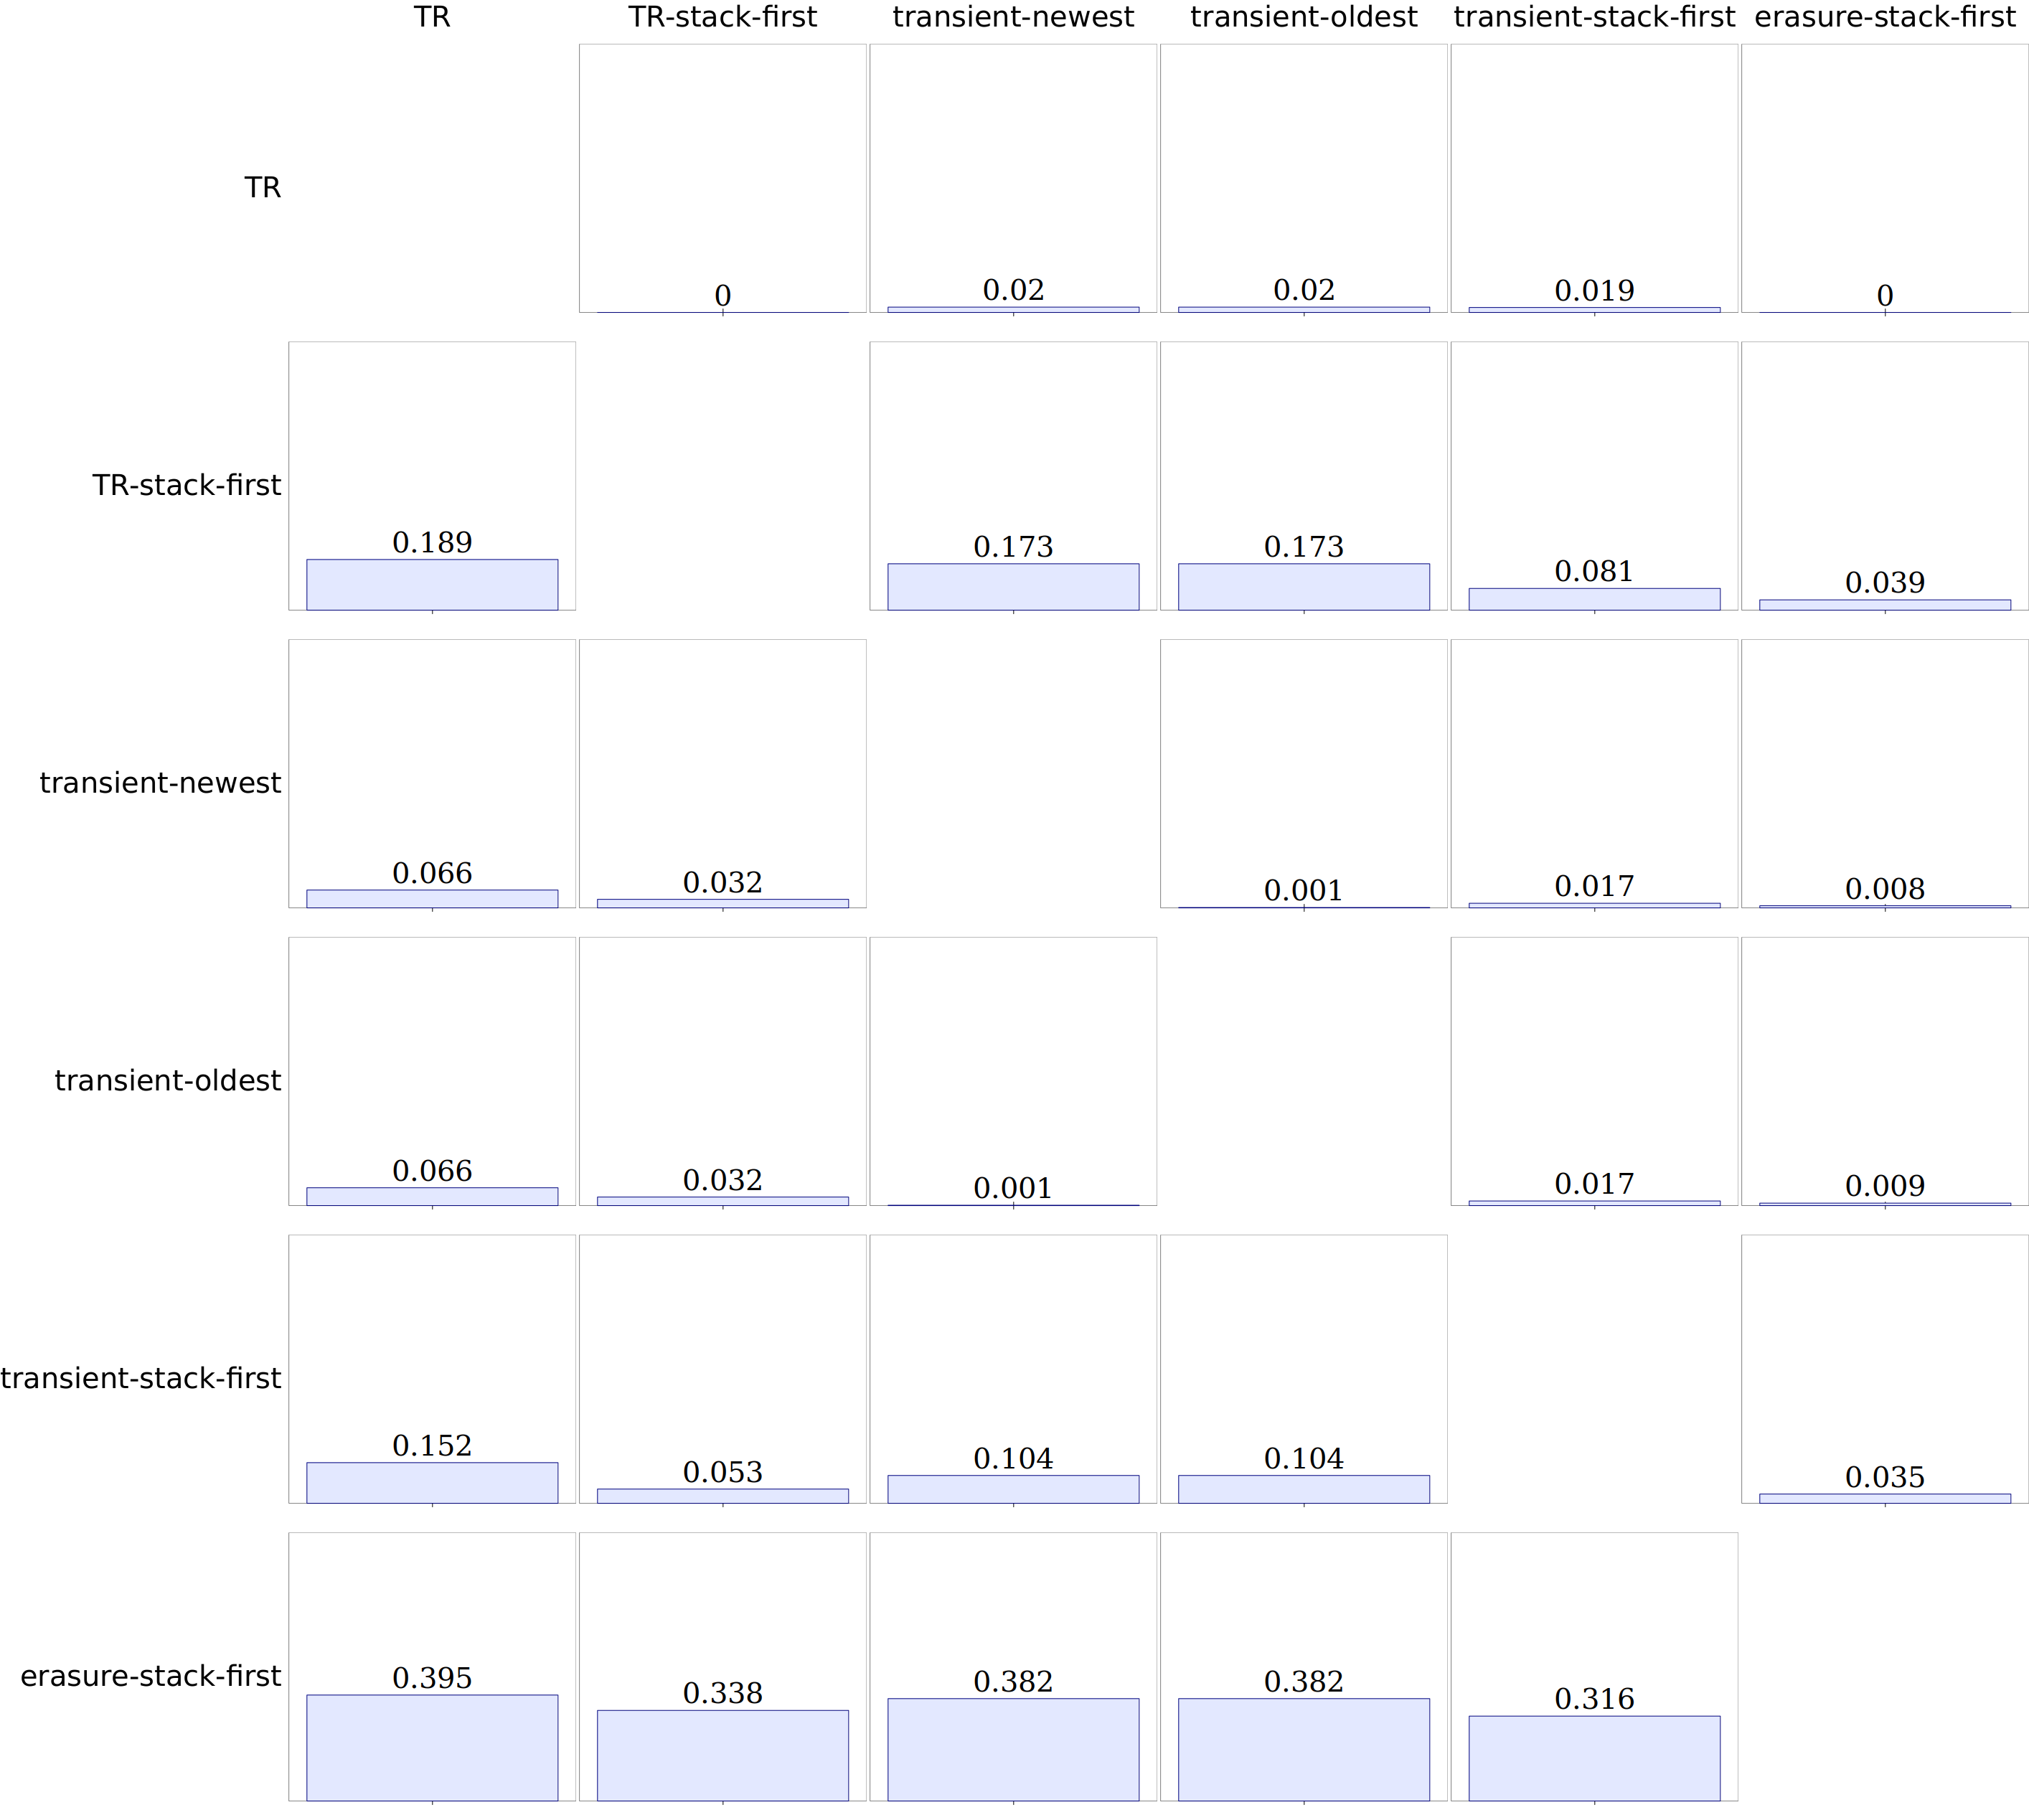
\includegraphics[width=0.45\textwidth]{./plots/avo-matrix}
  \caption{Usefulness comparisons: Each cell depicts the estimated percentage of
  interesting debugging scenarios for which the row mode is more useful
  than the column mode.
  The upper bound of error margin is 0.02\%}
  \label{fig:avo-matrix}
\end{figure}


\begin{figure}
  \centering
  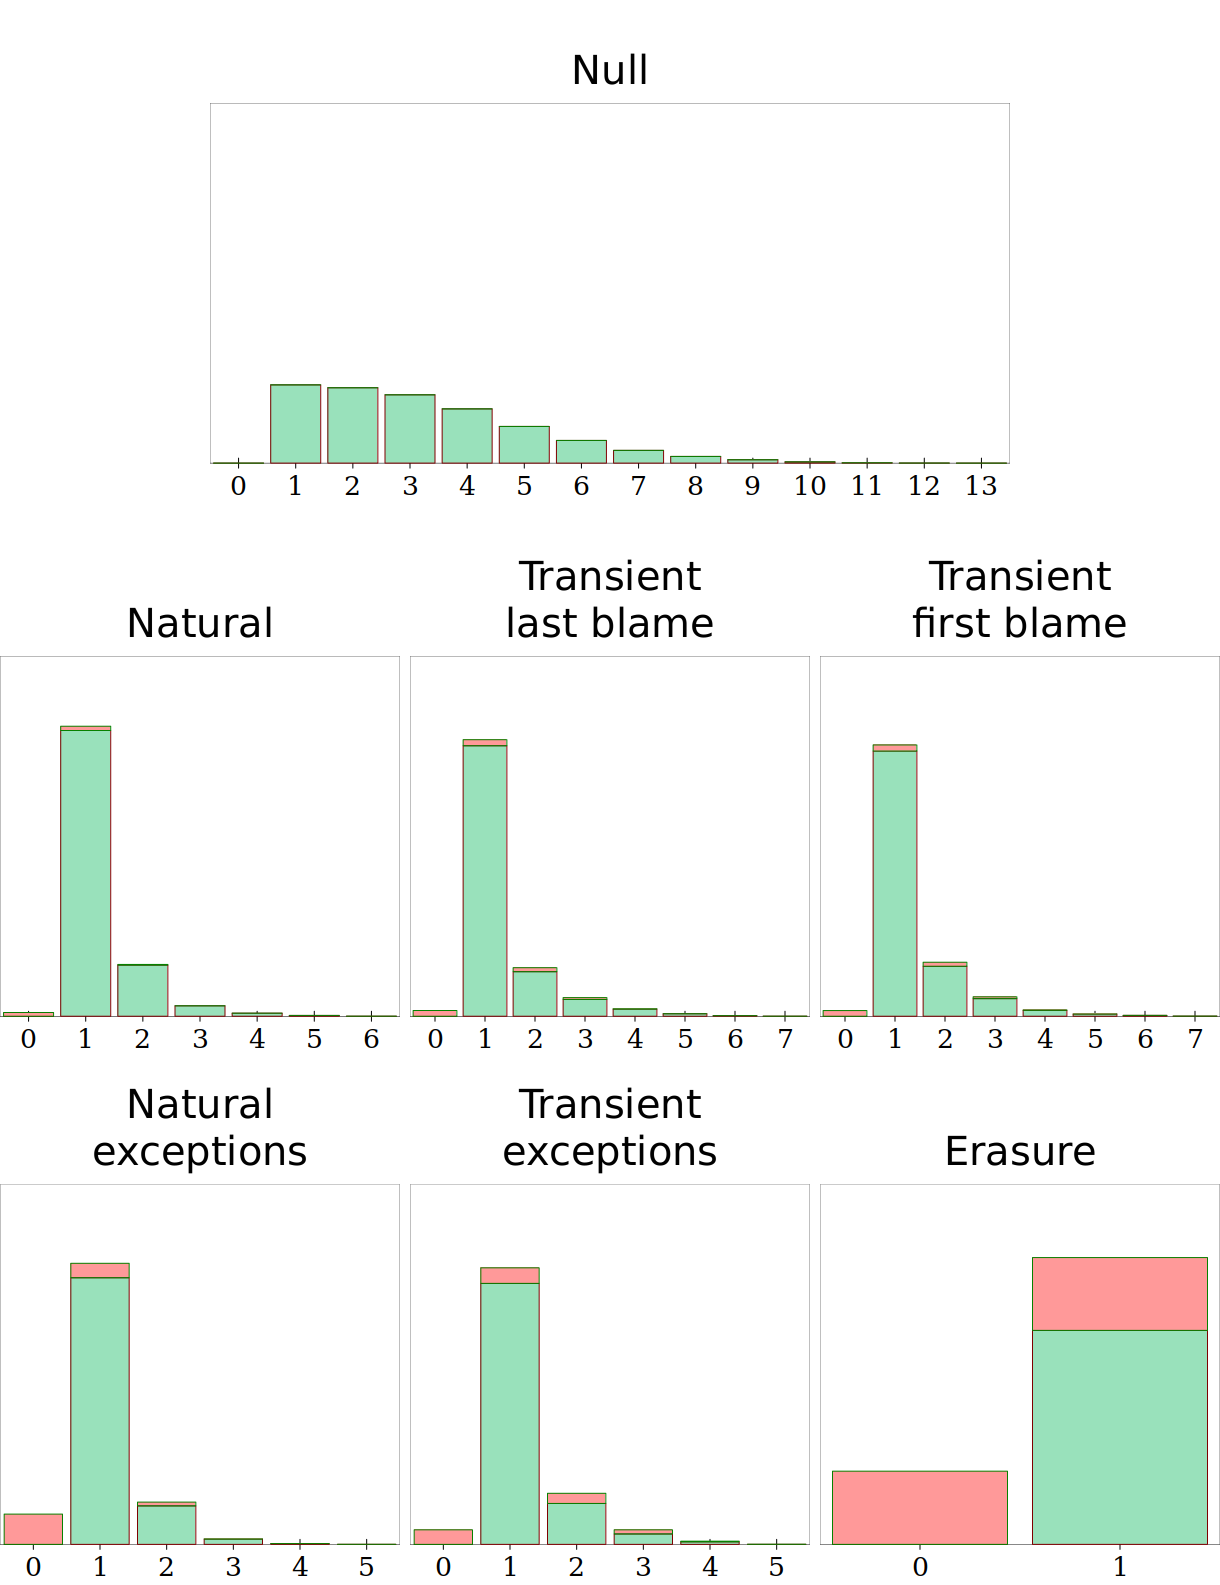
\includegraphics[width=0.4\textwidth]{./plots/bt-lengths-table}
  \caption{Programmer effort: Each plot depicts the distribution of trail
  lengths for a given mode across all benchmarks, starting from trails
  of length 0.}
  \label{fig:effort-table}
\end{figure}


Figure~\ref{fig:effort-table} shows the distribution of programmer effort
for our sample of interesting debugging scenarios. Unlike the usefulness
comparisons above, these proportions do not generalize to a representation of the full population.
Still, as we discuss in section~\ref{subsec:effort}, they provide an
alternative view of the workings of the rational programmer. 

There are
three immediate take-aways from the figure. First, the effort for successfully
debugging interesting scenarios (in green) for the random mode of the
rational programmer follows  a normal distribution, as expected.\footnote{The
random mode distribution is indistinguishable for all three semantics and thus the figure~\ref{fig:effort-table} 
only shows one plot.} In contrast, in the other modes, successful effort coalesces at
the left side of the plot, meaning that in most cases the programmer needs
to type a single component to debug a scenario. 

A second point of interest is that the exceptions of
the Erasure semantics either help the rational programmer immediately or 
the rational programmer fails to debug a scenario altogether (in red).
This is expected; no matter how many type annotations the programmer
adds to an Erasure program, if the type checker doesn't reject the
program, running the program always produces the same outcome. Thus an
exception from the runtime has to point to the buggy module with
the first try. Otherwise the rational programmer types an irrelevant
module, runs the program again and the exception points again to the
already typed module. 

A third notable piece of information from
the figure is that every mode has failed debugging scenarios, not just
Erasure. This should
not come as a surprise to the astute
reader. After all, as we
discuss above, some modes are more successful than others in certain
scenarios. Indeed any mode can fail if running a scenario results in an
exception and the exception carries no useful information about which
module the programmer should type next, e.g., because the stack trace 
does not contain frames from any module of the program, or only typed modules. This situation
can even happen immediately, which explains failures with 0 effort. 


While most failures to debug scenarios follow the above pattern, a few do not.
Breaking down the reasons for failure for Natural blame (1748 in total)
reveals an additional cause. For a small set of
debugging scenarios (40), Natural produces a run time type error
blaming a non-buggy already typed
component. We tracked down all these cases to known open issues with Typed
Racket and class contracts. 

In Transient, similar to Natural,
most failures are due to unhelpful exception information (1851 for both
Transient first and last blame).  
However, Transient also has a substantial
number of failures because scenarios hit the time and memory
limits of our experiment (~ 770 scenarios).  Additionally, there are nearly a 1000 cases where
Transient reports an empty blame set which leaves the rational programmer
without hints about how to proceed.
In~\ref{sec:threat:transient}, we discuss how both of these causes of
failure for Transient affect our experiment. 

      \label{sec:results}
%% -----------------------------------------------------------------------------
Interpreting the numeric summaries and aggregations of the preceding section
demands an intuitive understanding of what blame trails look like in practice.
A concrete example of blame trails and programmer modes is a good basis for
synthesizing this kind of intuition.

\begin{figure}
{
  \definecolor{trans-fb}{RGB}{215, 48, 31}
  \definecolor{trans-lb}{RGB}{252, 141, 89}
  \definecolor{trans-exn}{RGB}{253, 204, 0}
  \definecolor{erasure}{RGB}{119, 87, 254}

  \newcommand\config[1]{\begin{minipage}{0.09\textwidth}\centering\includegraphics[width=\linewidth]{Images/#1}\end{minipage}}
  \newcommand\runtimeError{\begin{minipage}{0.03\textwidth}\centering
\includegraphics[width=\linewidth]{Images/runtime-error}\end{minipage}}
  \newcommand\checkFailure{\begin{minipage}{0.03\textwidth}\centering
\includegraphics[width=\linewidth]{Images/check-failure-plain}\end{minipage}}
  \newcommand\blameFinger{\begin{minipage}{0.02\textwidth}\centering\vspace{0.25em}
\includegraphics[width=\linewidth]{Images/finger}\end{minipage}}
  \newcommand\typeError{\scalebox{1.5}{$\tau_{\hspace{-0.1em}\times}$}}
  \newcommand\success{\textcolor{black!30!green}{\checkmark}}
  \newcommand\fail{\textcolor{red}{\sffamily x}}
  \footnotesize
\centering
\begin{tabular}{l|ccl|ccl|cc|c}
\multicolumn{3}{c}{\begin{minipage}{0.25\textwidth}\centering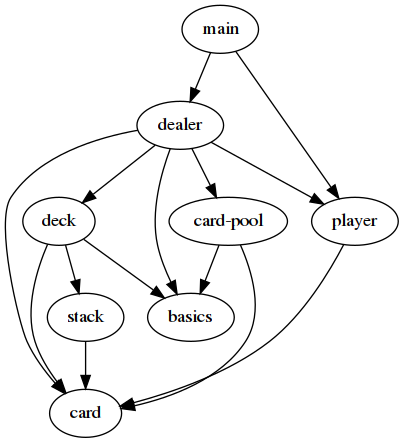
\includegraphics[width=\linewidth]{Images/take5-module-graph}\end{minipage}} &
\multicolumn{7}{c}{\begin{minipage}{0.69\textwidth}\centering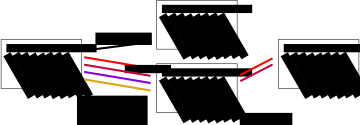
\includegraphics[width=\linewidth]{Images/trails-example}\end{minipage}} \\
\multicolumn{3}{c}{\begin{minipage}{0.25\textwidth}\centering the dependency graph\end{minipage}} &
\multicolumn{7}{c}{\begin{minipage}{0.69\textwidth}\centering the paths taken by each mode through the configuration lattice\end{minipage}} 
\vspace{1em} \\
\end{tabular}

\begin{tabular}{l|ccl|ccl|cc|c}
 & \textbf{Root} &  &  & \textbf{Step 1} &  &  & \textbf{Step 2} &  & \textbf{Success?}\\
\textbf{Mode} & config & result & stack & config & result & stack & config & result & \\
\hline
Natural & \config{10001100} & \blameFinger & \texttt{main} & \config{10001110} & \typeError &  &  &  & \success\\
-blame &  & \texttt{player} & \texttt{main} &  &  &  &  &  & \\
\hline
\textcolor{trans-fb}{Transient} & \config{10001100} & \runtimeError & \texttt{dealer} & \config{10011100} & \blameFinger & \texttt{dealer} & \config{10011110} & \typeError & \success\\
\textcolor{trans-fb}{-first-blame} &  &  & \texttt{dealer} &  & \texttt{player} &  &  &  & \\
\emph{and} &  &  & \texttt{dealer} &  & \texttt{dealer} &  &  &  & \\
\textcolor{trans-lb}{-last-blame} &  &  & \texttt{main} &  &  &  &  &  & \\
\hline
\textcolor{erasure}{Erasure} & \config{10001100} & \runtimeError & \texttt{dealer} & \config{10011100} & \runtimeError & \texttt{dealer} &  &  & \fail\\
 &  &  & \texttt{dealer} &  &  & \texttt{dealer} &  &  & \\
 &  &  & \texttt{dealer} &  &  & \texttt{dealer} &  &  & \\
 &  &  & \texttt{main} &  &  & \texttt{main} &  &  & \\
\hline
\textcolor{gray}{Natural} & \config{10001100} & \checkFailure & \texttt{main} &  &  &  &  &  & \fail\\
\textcolor{gray}{-exceptions} &  &  & \texttt{main} &  &  &  &  &  & \\
\hline
\textcolor{trans-exn}{Transient} & \config{10001100} & \runtimeError & \texttt{dealer} & \config{10011100} & \checkFailure & \texttt{dealer} &  &  & \fail\\
\textcolor{trans-exn}{-exceptions} &  &  & \texttt{dealer} &  &  &  &  &  & \\
 &  &  & \texttt{dealer} &  &  &  &  &  & \\
 &  &  & \texttt{main} &  &  &  &  &  & \\
\end{tabular}

\begin{minipage}{0.95\textwidth}
\vspace{0.5em}
\centerline{\it Legend}

\noindent{\bf config} Each box corresponds to a module and indicates (with x) if it is typed. 
The mutated module is gray.

\medskip

\noindent{\bf result}\\
\begin{center}
\begin{tabular}{l@{\quad}l}
symbol        & denotation \\ \hline 
\blameFinger  & the configuration results in a dynamic type-check failure, blaming the module(s) below \\
\typeError    & the configuration does not type check\\
\runtimeError & the configuration fails a check to the runtime system\\
\checkFailure & the configuration signals a dynamic type check failure for which blame is ignored\\
\end{tabular}
\end{center}

\end{minipage}}


\caption{An example scenario from take5, with every mode's resulting trail.}
\label{fig:example-trails}
\end{figure}

Figure~\ref{fig:example-trails} summarizes one particularly interesting
debugging scenario from the {\tt take5} benchmark. The module dependency graph
of this benchmark is shown in the top left of the figure. Its mutated {\tt
player} module provides a method under a different name than the client module,
{\tt dealer}, expects. In Typed Racket's gradual type system, this mistake
corresponds to a type-impedance mismatch---and all rational-programmer modes
come to different conclusions. 

The rest of figure~\ref{fig:example-trails} illustrates the blame trails for
every mode of the rational programmer (except Random) for the debugging scenario
in two different ways:
\begin{itemize}

\item The top right shows the blame trails produced by every mode of the rational programmer as paths through the configuration lattice starting at the
root (leftmost) configuration. Each configuration is represented by a sequence of boxes corresponding to modules in the program, with an x indicating that the module is typed.
The mutated module has a gray box.

\item The table in the middle expands the information in the diagram with the details of every step in each trail.
Every row of the table represents the trail of one mode. The middle-three columns depict the steps of a blame trail:
\begin{description}
\item[Root] describes the result of running the root configuration in this row's mode.
\item[Step 1] is the result of the rational programmer's reaction to the outcome of running the root. 
\item[Step 2] shows the result of reacting to the outcome of running step~1 configuration, if any. 
\end{description}
Finally, the \textbf{Success?} column summarizes whether exploring the trail succeeds.

\end{itemize}

To make this table concrete, compare rows 1 and~4. The first one shows that
running the root configuration under the Natural-blame mode fails due a dynamic
type check and blames the {\tt player} module; typing that module and running
again then results in a type error, and hence the trail is successful.  By
contrast, the Natural-exceptions mode (row 4) yields stack information for the
root configuration that is unhelpful; it identifies only {\tt main}, which is
already typed. Hence, this trail immediately gets stuck.

In short, this figure concretely demonstrates how the rational programmer
behaves in different modes. In this case, the behaviors differ from each other
in five of the six modes (the two Transient blame modes behave the same).
The reader may keep these scenarios for the following discussion of the numeric results.

\subsection{Interpreting the results}

The results of the experiment suggests a number of high-level conclusions about
blame strategies in the gradual typed world.  First, run-time type checks have a
large positive impact, regardless of whether these checks assign blame or throw
plain exceptions.  Second, error messages with blame assignments are more
helpful than those without. The results also indicate, though, that blame is not
critical in a majority of cases, and therefore they suggest investigating
whether blame tracking is worth the performance cost.  Third, the Natural
approach fares better than the Transient approach, but only by a small margin.
Since Natural offers complete and sound path-based blame  while Transient offers
incomplete but sound heap-based blame~\citep{gfd-oopsla-2019}, the results call
for a study concerning the relative strengths of the two models of blame.
Fourth, given that Transient's sound but shallow run-time type checks do not
seem to hamper debugging, a language that supports {\em both\/} Natural and Transient 
might help reduce the number of wrappers and thus address the well-known
performance issues of sound gradual typing~\citep[chapter~6]{g-dissertation-2020}.  Fifth, the fact that both
modes of the Transient rational programmer are equally successful suggests that
returning the whole blame sequence may not be beneficial. If so, Reticulated
Python could limit the size of blame sequences to attempt to mitigate its
serious performance problems (see below).

%% -----------------------------------------------------------------------------
\subsection{What Are the Threats to Validity?}

The validity of these conclusions is threatened in two fundamentally distinct
ways. The first sets of threats have been mentioned before: (i) the
representativeness of benchmarks; (ii) the relation between mutations and real
programming mistakes; and (iii) the sampling strategy.  While the experimental setup attempts to
mitigate against these threats, the reader must definitely take into account
these limitations of the experiment and must understand that the collected data
not support any further generalization.

The second set of threats connects the experiment with reality or, more
precisely, assess how close the connection is. To start with, it questions the
realism of the rational programmer itself (sec.~\ref{sub:rational}), followed by
the definition of ``interesting scenarios''
(sec.~\ref{sec:threat:erasure-bias}).  The remaining questions address the
accuracy and the cost of Transient blame, respectively (see
secs.~\ref{sec:threat:transient} and~\ref{sec:threat:transient2}).

%% -----------------------------------------------------------------------------
\subsection{Threat: Is the Rational Programmer Realistic?} \label{sub:rational}

Like {\em homo economicus\/}, which idealizes the actual behavior of a
participant in an economy for the sake of mathematical modeling, the model of a
rational programmer idealizes the actual debugging behavior of a software
developer for the sake of a systematic, large-scale analysis. This idealization 
comes with advantages and disadvantages. In the economic realm, mathematical
models have provided some predictive insights into the market's behavior; but as
behavioral economics has shown more recently~\cite{henrich2001search},
the mathematical abstraction of a
rational actor makes predictions also quite unreliable in some situations.
\footnote{It has misled economists to focus on just mathematics, though
this problem is not relevant here---tongue firmly in cheek.}  Just like an
ordinary consumer or producer, an actual software developer is unlikely to stick
to the exact strategy proposed here. When this happens, the predicted benefits
of blame assignment may not materialize. Indeed, the authors' personal
experience suggests such deviations, and it also suggests that deviating often leads to dead-ends.
To make a true judgment of the usefulness of the rational-programmer
idea, the community will need much more experience with this form of evaluation
and relating the evaluation to the behavior of working programmers.

Relatedly, the experimental setup hides how a rational programmer ascribes types
to extend a trail. When the run-time checks signal an impedance mismatch in the
real world, a programmer does not have a typed module ready to swap
in. Instead, the programmer must come up with the next set of types, which means
making choices. It is usually possible to consistently assign types to variables
in a module in several different ways. The maintenance of the benchmarks over many years
has driven home this lesson but, fortunately, it has also shown that the types
are in somewhat canonical.  The authors therefore conjecture that different
real-world programmers would often come up with equivalent type assignments
during debugging sessions. 

%% -----------------------------------------------------------------------------
\subsection{Threat: Is the Definition of Interesting Scenarios Reasonable?} \label{sec:threat:erasure-bias}

Section~\ref{sub:mutate-interesting} defines criteria for interesting mutations,
one of which limits the scenarios under consideration to those with mistakes
that raise a run-time error under Erasure. In other words, the experiment is
Erasure-biased: it only considers the usefulness of blame when the safety checks
of the underlying language alone are sufficient to detect the mistake. In
reality, some mistakes require run-time type checks to be
detected~\cite{gfd-oopsla-2019}, and it is possible that blame has more 
to offer for these kinds of mistakes. If that is the case, then the results of
the experiment on a population of scenarios including such mistakes should be
different.

In fact, a variation of the experiment provides
some preliminary evidence that this difference may be significant. Thus far,
the variation of the experiment covers only three of the
benchmarks but broadens the selection of scenarios to include any that raise
run-time errors under Natural, regardless of other semantics. The 
results from this small experiment suggest that without Erasure-bias, Natural blame
may be much more useful than all of the other modes.

%% -----------------------------------------------------------------------------
\subsection{Threat: Why Does Transient Lose Blame?} \label{sec:threat:transient}

The execution of the experiment reveals that Transient produces empty blame
sequences for 967 scenarios. An empty blame sequence means a lack of boundary
crossings for the witness value. In theory, an empty sequence should not occur,
because it means a typed module is blaming itself---something that can happen only
if the type checker (or system) is unsound.

An investigation of these empty blame cases reveals that Transient is not
unsound but that Vitousek et al.'s Transient blame assignment loses track
of the proper boundaries due to an incomplete initialization of the blame map.
Despite these losses, the number of failures is a small fraction of the
overall number of debugging scenarios. It is unlikely that any
improvements to Vitousek et al.'s strategy would change the overall
conclusion about Transient blame.

{\bf Note} The scenarios where Transient returns no blame suggest two ways to
improve its blame map.  First, entries in a blame map should point to {\em
several\/} parent entries.  For example, if \texttt{f} receives bad input in the
context of {\tt (filter f xs)}, the entry should point to both \texttt{filter}
and \texttt{xs}. Second, the construction of entries must be guided by type-like
specifications for primitives instead of special cases for built-in
functions. Aliasing such function changes the blame map.  


%% -----------------------------------------------------------------------------
\subsection{Threat: Is the Transient Blame Assignment Mechanism Realistic?}
\label{sec:threat:transient2}

The results in section~\ref{sec:results} also show that the cost of Transient
blame is quite high. Under the Transient semantics, some of the debugging
scenarios exceed the 4-minute timeout or the 6GB-memory limit. To put those
limits into context, the fully typed and fully untyped benchmarks all normally complete
in a few seconds with minimal memory usage. Furthermore, none of the mixed
Natural configurations hit these limits, and with the blame map turned off,
the Transient semantics also runs these programs in a short amount of time and
well within the memory limit. In short, even though the Transient rational
programmer appears to do well in the experiment, the implementation of the
Transient blame strategy might be unrealistic. 

At first glance, these measurements seem to contradict the results
of~\citet{vss-popl-2017}. They report an average slowdown of 6.2x and a
worst-case slowdown of 17.2x on the fully-typed Python benchmarks in Reticulated
Python when the blame map gets enabled.  Unfortunately, the average slowdown of
133x and the worst-case slowdown of 560x due to blame in Shallow Racket seems
closer to the truth.  There are at least three broad factors that skew Vitousek
et. al.'s results:
\begin{enumerate}

\item The 2017 implementation of Reticulated fails to insert certain soundness
checks\footnote{Missing check:
\url{https://github.com/mvitousek/reticulated/issues/36}} and blame-map
updates\footnote{Missing cast:
\url{https://github.com/mvitousek/reticulated/issues/43}} from the paper.

\item While Reticulated attempts to infer types for local variables, the impoverished nature of its type
    system does not allow the ascription of precise types and often resorts
    to type {\tt Dynamic}~\citep[section~5.4.4]{g-dissertation-2020}. 
    Code with type {\tt Dynamic}
    has fewer constraints to check at run-time---and much less information
    to track in the blame map.

\item \citet{vss-popl-2017} use small benchmarks.  Four have since been retired
from the official Python benchmark suite because they are too small,
unrealistic, and unstable.\footnote{Release notes:
\url{https://pyperformance.readthedocs.io/changelog.html}}  On the flip
    side, all the benchmarks in the GTP suite are larger than the official Python
    benchmarks. Reticulated Python  runs the
    translation of the smallest GTP benchmark in
    approximately 40 seconds without blame but times out after 10 minutes
    with blame.

\end{enumerate}
More work on Transient blame is needed to make an informed decision about
its prospects as a viable production-level approach. 


%% NOTE: Vitousek's benchmarks are from the Python "pyperformance" suite.
%%   The version notes in the docs talk about retiring benchmarks, but
%%   you can also look at the current codebase and see what names from POPL'17
%%   are missing: callsimple, callmethod, callmethodslots, & pystone
%% <https://github.com/python/pyperformance/tree/master/pyperformance/benchmarks>
   \label{sec:discussion}
\section{Related Work}
\label{sec:related}

This paper builds on~\citet{lksfd-popl-2020}'s one-of-a-kind analysis of
blame for higher-order contracts. They do not spell out the notion of the
rational programmer but the basic ingredients of our technique derive
directly from theirs. Specifically, we adapt their empirical technique
to gradual typing which requires the development of custom mutators,
careful selection of debugging scenarios and generalization of the
technique to allow the comparison of different semantics.

The literature on gradual typing presents many semantics beyond the three
that we study, but only two additional blame strategies.
Pyret (\shorturl{https://www.}{pyret.org}) treats fixed-size data types same as Natural
and functions same as Transient. The Forgetful~\cite{cl-icfp-2017} and
the Amnesic~\cite{gfd-oopsla-2019} semantics are similar to Transient but
use wrappers instead of inlined checks.  Nom~\cite{mt-oopsla-2017} and
other \emph{concrete\/} semantics~\cite{wnlov-popl-2010, rsfbv-popl-2015,
rzv-ecoop-2015, rat-oopsla-2017} assume that every value comes with a type tag
and use tag checks to supervise the interactions between typed and untyped code.
Monotonic
references~\cite{svctg-esop-2015} and the semantics~\cite{tlt-popl-2019,
etg-icfp-19, tt-scp-20, tgt-popl-18, tt-sas-17} derived with the
Abstracting Gradual Typing
technique~\cite{gct-popl-2016} are (optimized) variants of Natural.
Among these representative semantics, only Amnesic and Nom present innovative
blame strategies.
Our study nevertheless excludes these strategies because Amnesic is a mere
theoretical construction and Nom imposes restrictions on untyped
code that would necessitate new data definitions across our benchmarks.
 
      \label{sec:related}
%% -----------------------------------------------------------------------------
\section{What to Do Next} 

The paper provides the first insight into the measurable value of blame
 in the gradually typed world. In an implicit manner researchers and
language designers have answered this question one way or another, without any
evidence. Now they may use the evaluation method of this paper to
confirm or reject their answers. We already know from~\citet{tgpk-dls-2018}
that, by intuition, programmers prefer the run-time checking of natural over
other soundness methods. But, just because a random set of programmers expresses
this view does not mean that blame assignment adds value. At this point we know
that it does, in some circumstances, and that in others, the answer remains
murky.

The paper does {\em not\/} address a problem in the gradually typed world that
was pointed out early on by practical researchers~\cite{incorrect-ts,
sta-nt-base-types, wmwz-ecoop-2017} and that has recently received theoretical
attention~\cite{gfd-oopsla-2019, cc-oopsla-20}: mistakes in type annotations themselves.
Developers use gradual typing to move an untyped code base into the typed realm,
and to this end, they need typed APIs for the vast repositories of
already-existing libraries. Because they can, language implementors merely
create typed facade modules that import untyped functions and export them with
type annotations---instead of converting the libraries themselves. With those
facades, the compiler can easily type-check typed components. Problem is
that these retroactive additions of types to a library may result from a misunderstanding of the
code. \emph{They may thus be a mistake themselves.}

The cited evidence suggests that this scenario is quite common and largely unadressed.
%, and that a type soundness check does {\em not\/} at all address the problem.  
Hence, a future evaluation must develop type-level mutators that produce incorrect type
annotations without breaking the code itself. Some preliminary work suggests
that such type mutators are much more difficult to develop than the code
mutators of this paper. We conjecture that the natural semantics will
usually discover such mistakes, while the transient and erasure semantics cannot
help with such mistakes at all; indeed, we expect that these latter two raise
misleading exceptions or produce plainly-wrong answers.  Of course, only further
evaluation work can confirm or reject these conjectures.



   \label{sec:conclusion}

%% Acknowledgments
%%\begin{acks}                 
  %% acks environment is optional
  %% contents suppressed with 'anonymous'
  %% Commands \grantsponsor{<sponsorID>}{<name>}{<url>} and
  %% \grantnum[<url>]{<sponsorID>}{<number>} should be used to
  %% acknowledge financial support and will be used by metadata
  %% extraction tools.
%%\end{acks}


%% Bibliography
\bibliography{cs}

\end{document}
